%\begin{figure}
%  \begin{center}
%  \includegraphics[width=0.8\textwidth]{Chart_of_Nuclides.pdf}
%  \caption{Figure caption}
%  \label{chart}
%  \end{center}
%\end{figure}

\epigraph{``The grandest discoveries of science have been but the rewards of
    accurate measurement and patient long-continued labour in the minute
sifting of numerical results.''}{William Thompson, \nth{1} Baron Kelvin}

\section{Models of the atomic nucleus}

To unravel the nuclear many-body problem, we can
employ models that incorporate essential details while ignoring specifics with
little relevance to the observables we care about.

Liquid Drop Model

An especially simple and
effective model, the Liquid Drop Model (LDM), describes nuclei as drops of
an ideal nuclear fluid and has been successfully employed for many decades to
describe nuclear masses. The binding forces of each nucleus are modeled by five
physically-intuitive terms appropriate for such a fluid:

a volume term that describes "bulk" binding that would be experienced in an
infinite sea of nuclear matter, or  by completely surrounded nucleons in the core of the nucleus,

a surface term that incorporates the finite size of a nucleus (i.e., it is a
drop, not an ocean), equivalent to surface tension,

a coulomb term that incorporates the electric repulsion experienced by protons
constrained in close proximity to each other inside the drop,

an asymmetry term representing the relative chemical potential of neutrons and
protons as a function of their relative population (which can be re-balanced by
beta-decay),

and a spin-orbit term responsible for modeling the interaction of the intrinsic spin
of a nucleus and its constituent nucleons' angular orbital momentum, which is
a much stronger effect in nuclear binding than in the atomic case

In this model, each term is parameterized and the ensemble can be fitted to
well-measured nuclear masses across the chart of nuclides. Happily, though the detailed
quantum structure is completely ignored, these five terms are quite successful
in describing nuclear masses.

The Independent Particle Model (IPM) provides a complementary approach expressly
focused on the quantum details of the problem. The many-body problem is
approximated by considering each nucleon as moving independently of all other
nucleons in an potential generated by those nucleons. As in the atomic case,
where electrons obey an aufbau principle and populate orbitals defined by the
atomic potential, both protons and neutrons obey a nuclear aufbau, filling
orthogonal states in the nuclear potential. In this model, many fundamental
quantum properties of nuclei are easily understood, (for example, ground state spins and
the appearance of shell closures in direct analogy to the atomic case).
Unfortunately, the assumption of independent nucleon motion that defines the model
also kneecaps its usefulness: in reality, nuclear systems are strongly
correlated and exhibit clustering and collective motion, behaviors at odds with the
the IPM picture.

Additional models (RPA, Density Functional Theories, Optical Models

Optical Model description of the nucleus
-> can largely follow Bob and Wim's review paper
- first formulated in 1949 to describe neutron cross section data
- separate proton and neutron global optical potentials in the 60s (Becchetti
and Greenlees)
- CH89 includes additional neutron scattering data on isotopic targets

Takeaway: neutron scattering data particularly valuable for constraining these
models, but particularly challenging to access experimentally.

"The magnitude and energy dependence of the real isovector part of the
optical potential are poorly constrained by experiment." \cite{Holt16}

Hodgson's optical model review in 1971

Lane potential 

Isovector versus isoscalar. Charged pion exchange mediates the isovector forces;
other nucleon-nucleon interactions mediate the isoscalar forces.

Connect to Vinas, Chuck Horowitz, and J. Piekarewicz's neutron star EOS work.

Connect to chiral effective field theory work for calculating optical potentials
and examining isovector component of potential, especially w/r/t to exotic
nuclei near driplines.

Connect to FRIB/study of extremely neutron-rich systems relevant for r-process
and astrophysical nucleosynthesis.

At end of introduction:
- familiar with optical model historical development and current issues
- familiar with value of neutron scattering data for optical models and also as
fundamentally valuable for nuclear science
- familiar with scarcity of certain types of difficult neutron and proton
scattering data (\tot, \rxnE)
- familiar with relevance to infinite nuclear matter equation of state and
neutron star radii

\begin{figure}
    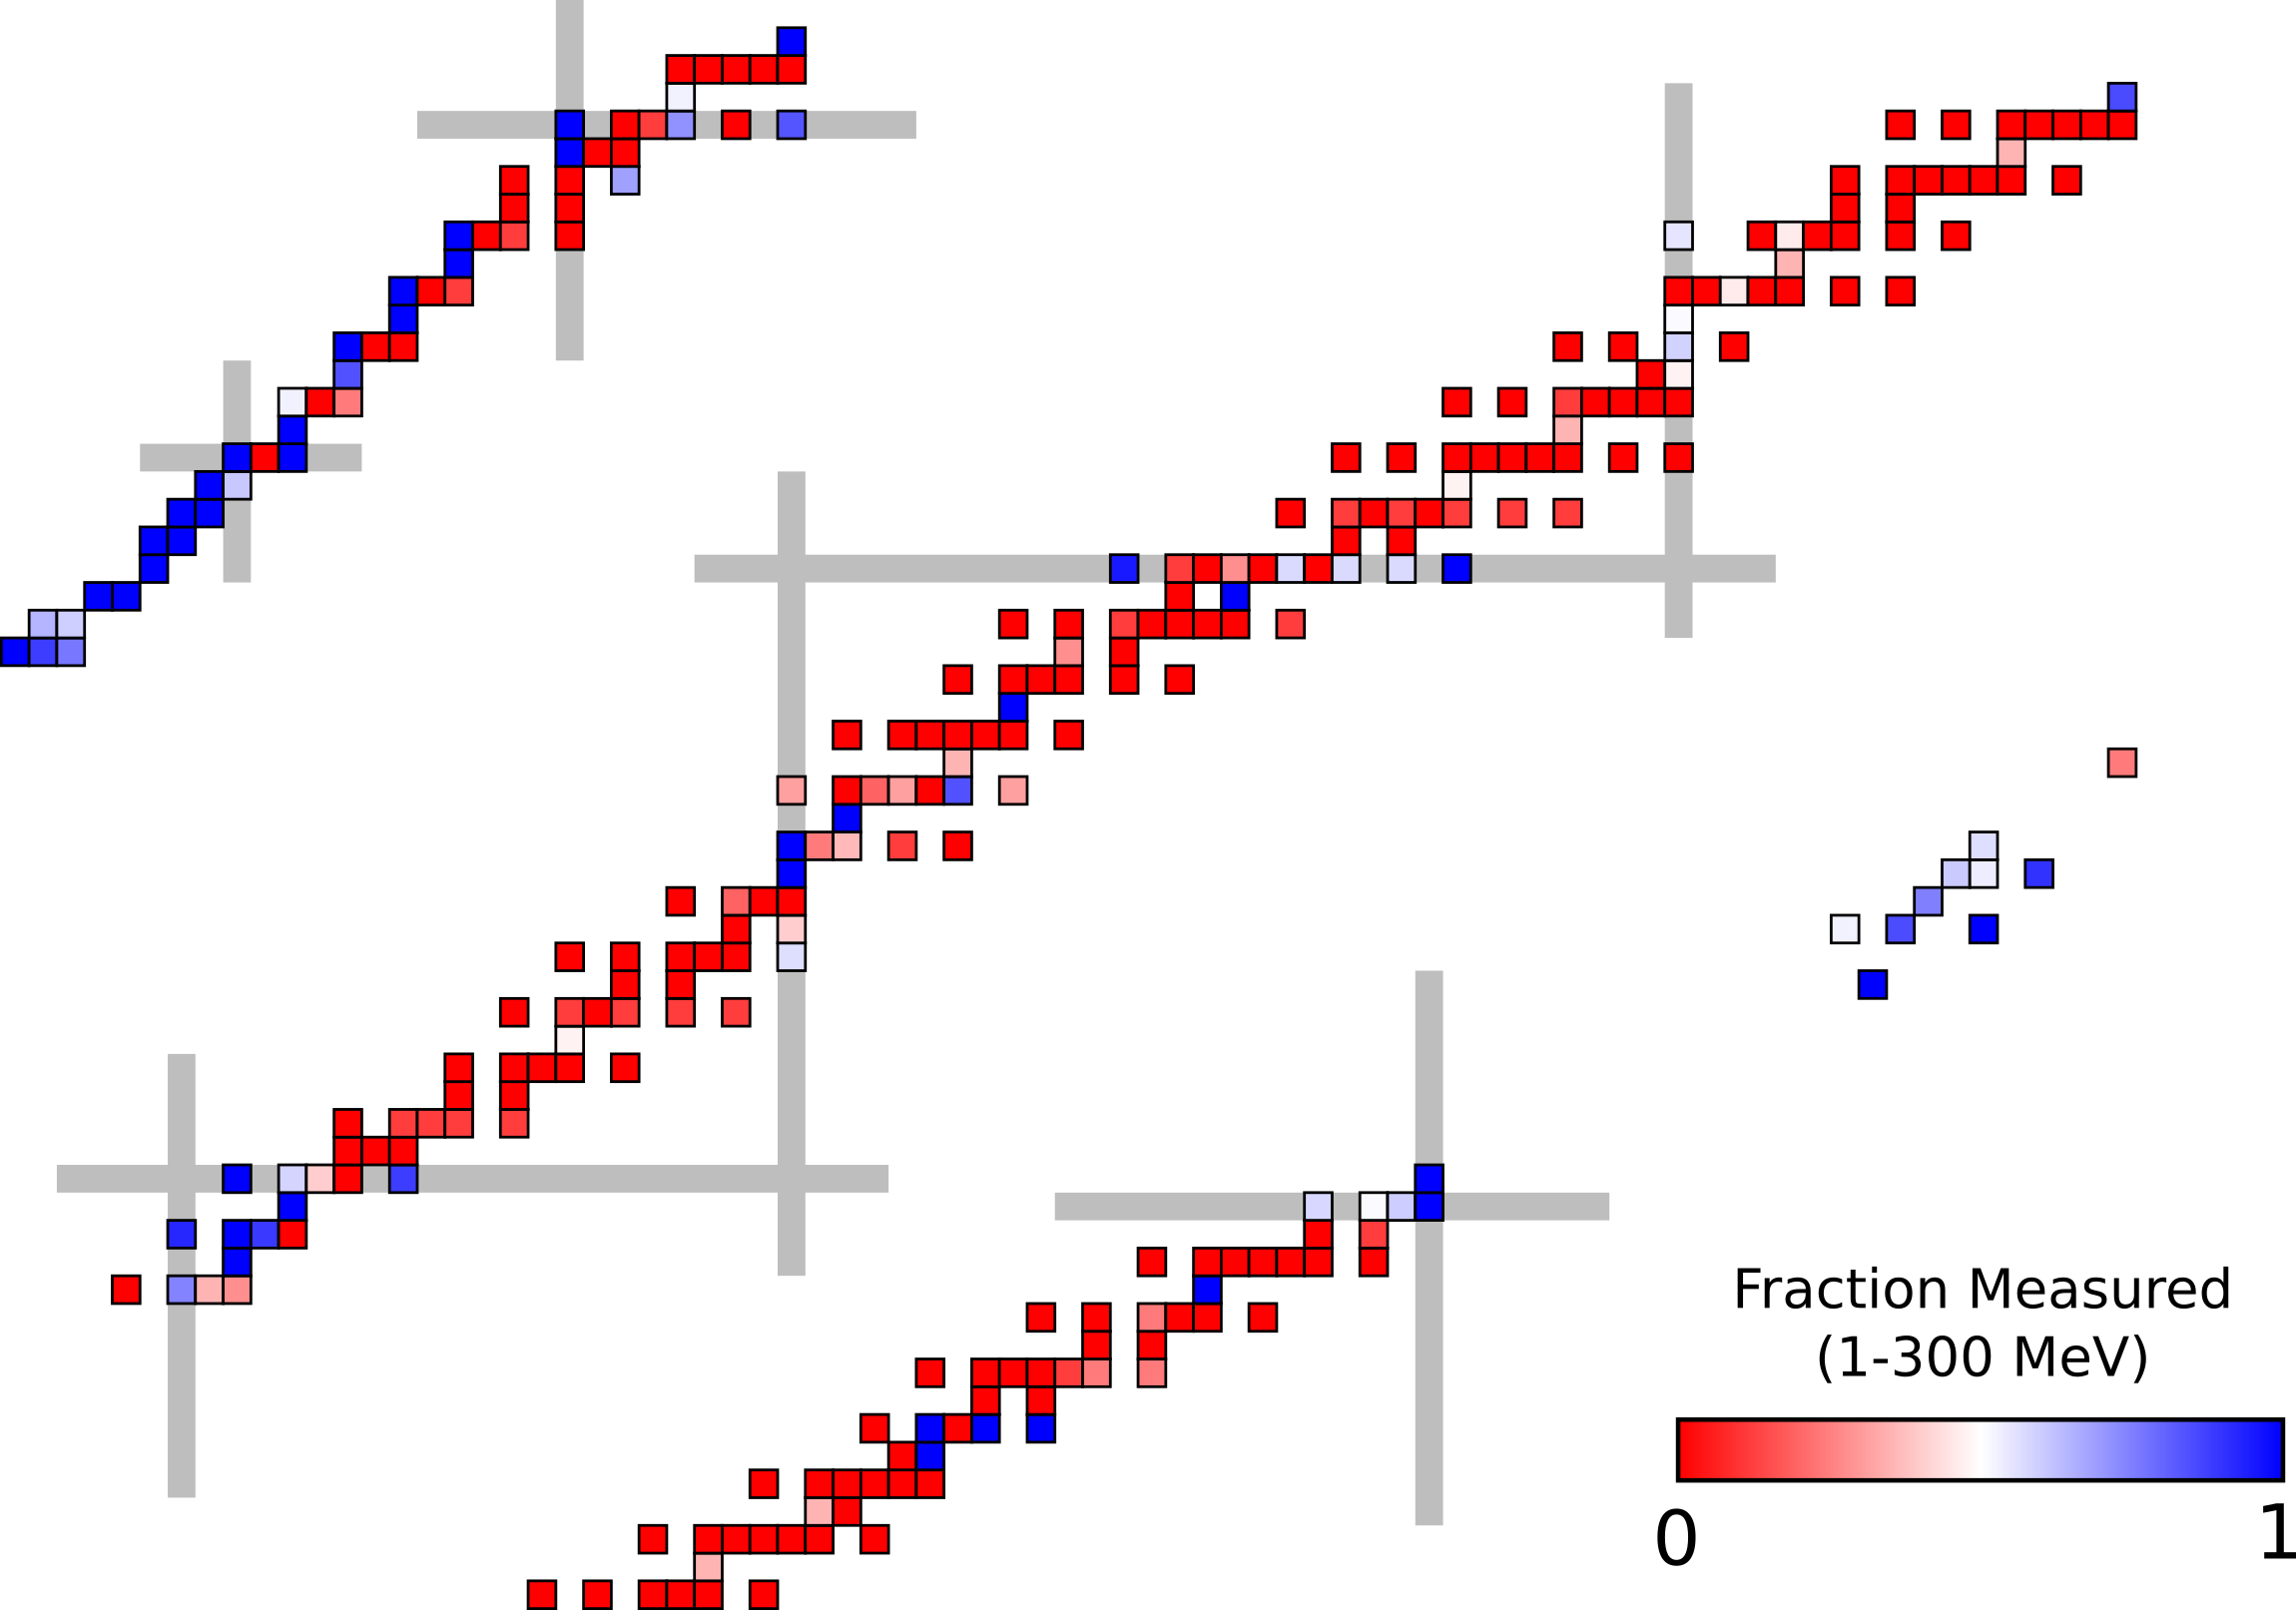
\includegraphics[width=0.8\textwidth]{figures/TCSChart.png}
    \caption{Figure caption}
    \label{chart}
\end{figure}

\begin{figure}
    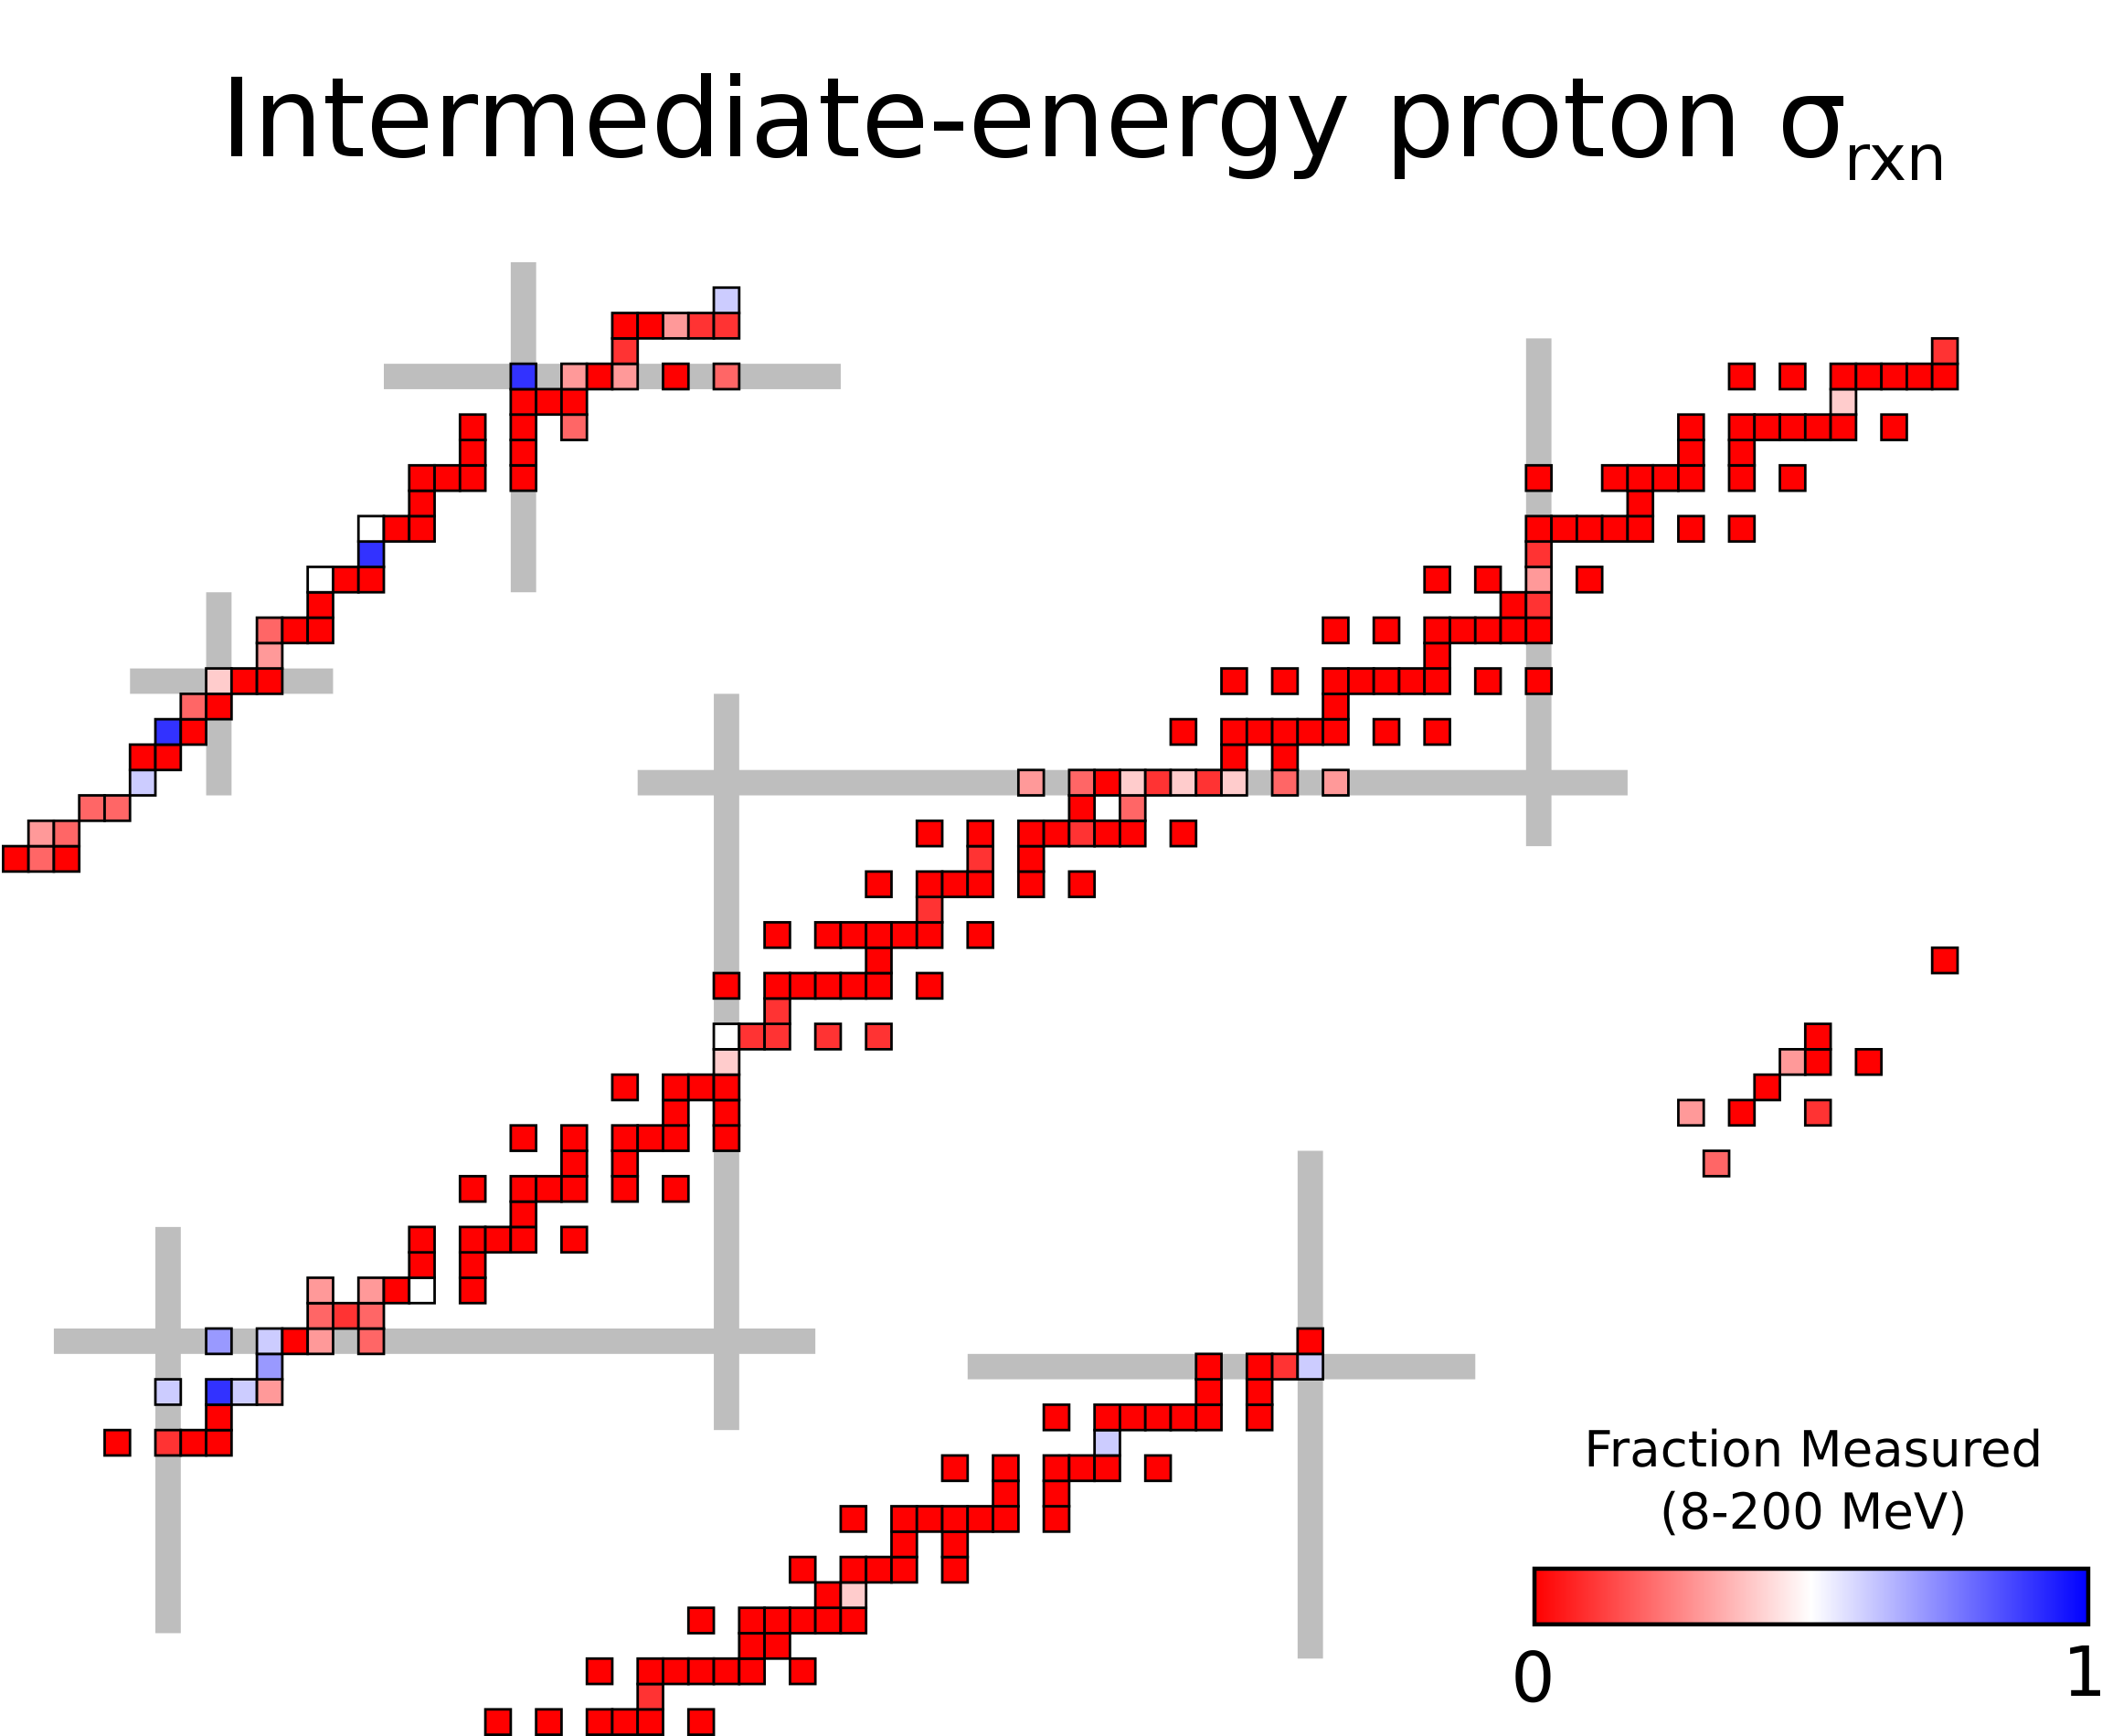
\includegraphics[width=0.8\textwidth]{figures/RCSChart.png}
    \caption{Figure caption}
    \label{chart}
\end{figure}

% \Gls{DOM} for glossary term
% \noindent for no indent

%\begin{comment}
% Woods-Saxon potential 
%\end{comment}
%
%\begin{equation}
%V(r) = \dfrac{-V_0}{1+e^{(r-R)/a}},
%\end{equation}

%\mathbf{J} = math bold-font symbol 'J'
